\documentclass[crop,tikz]{standalone}
\usepackage{tikz-3dplot}
\usepackage{pgfplots}
\makeatletter
\usetikzlibrary{3d, arrows.meta, bending, decorations.markings}
\usepgfplotslibrary{polar}
\pgfplotsset{compat=newest}


\makeatletter \newcommand{\pgfplotsdrawaxis}{\pgfplots@draw@axis} \makeatother

\pgfplotsset{axis line on top/.style={
  axis line style=transparent,
  ticklabel style=transparent,
  tick style=transparent,
  axis on top=false,
  after end axis/.append code={
    \pgfplotsset{axis line style=opaque,
      ticklabel style=opaque,
      tick style=opaque,
      grid=none}
    \pgfplotsdrawaxis}
  }
}



\begin{document}


% kepler_2_particles
\tdplotsetmaincoords{70}{110}
  \begin{tikzpicture}[scale=4, tdplot_main_coords]
  	
    \coordinate (O) at (0,0,0);
    \draw[thick] (-1.5,0,0) -- (O);
    \draw[thick] (0,-1,0) -- (O);
    \draw[thick] (0,0,-0.75) -- (O);
    \draw[->, >=latex, thick] (O) -- (1.5,0,0) node[anchor=north east, yshift=1mm]{$X$};
    \draw[->, >=latex, thick] (O) -- (0,1,0) node[right]{$Y$};
    \draw[->, >=latex, thick] (O) -- (0,0,0.75) node[left]{$Z$};
    
    % Define coordinates of the two bodies
    \pgfmathsetmacro{\px}{0.5};
    \pgfmathsetmacro{\py}{-0.9};
    \pgfmathsetmacro{\pz}{0.5};
    \pgfmathsetmacro{\dx}{-1};
    \pgfmathsetmacro{\dy}{0.8};
    \pgfmathsetmacro{\dz}{0.3};
    \coordinate (M1) at (\px,\py,\pz);
    \coordinate (M2) at (\dx,\dy,\dz);
    
    % Draw the bodies
    \fill[fill=blue!50!black!50] (M1) circle (1pt);
    \fill[fill=red!50!black!50] (M2) circle (1pt);
    
    % Draw the positions of each body relative to the origin
    \draw[->,>=stealth] (O) -- (M1) node[pos=0.7, above, yshift=1mm]{$\mathbf{r}_1$};
    \draw[->,>=stealth] (O) -- (M2) node[pos=0.7, above, yshift=1mm]{$\mathbf{r}_2$};
    
    % Draw the projections of both bodies onto the plane
    \draw[dashed] (M1) -- (\px, \py, 0);
    \draw[dashed] (\px, \py, 0) -- (0, \py, 0);
    \draw[dashed] (\px, \py, 0) -- (\px, 0, 0);
    \draw[dashed] (M2) -- (\dx, \dy, 0);
    \draw[dashed] (\dx, \dy, 0) -- (0, \dy, 0);
    \draw[dashed] (\dx, \dy, 0) -- (\dx, 0, 0);
    
    
    %% Draw the vector from body 1 to body 2
    %\draw[->,>=stealth] (M1) -- (M2) node[pos=0.6, above]{$\vec{r}$};
    
    % Provide the masses
    \node at (M1) [left, xshift=-0.75mm]{$m_1$};
    \node at (M2) [right, xshift=1mm]{$m_2$};
  \end{tikzpicture}

\newpage
% reduced_mass_system
\tdplotsetmaincoords{70}{110}
  \begin{tikzpicture}[scale=4, tdplot_main_coords]
	% Draw a sample trajectory that the particle takes
	\begin{scope}
		% Draw "rings" where the trajectory "passes through the horizontal plane"
		\foreach \t in {49.25, 149.4} {
			\pgfmathsetmacro{\x}{2-cos(\t)^2}
			\pgfmathsetmacro{\y}{-0.35*cos(\t)+\t/180}
			\pgfmathsetmacro{\z}{cos(\t)^2-0.1*sin(\t)}
			\begin{scope}[canvas is xy plane at z=\z]
				\draw[red!80!black!80] (\x,\y) circle (0.2 mm);
 			\end{scope}
 		}
 		
		% Define times at which the trajectory looks like it passes through
		% the planes
		\pgfmathsetmacro{\tlim}{105}
		\pgfmathsetmacro{\tlimTwo}{198}
		\pgfmathsetmacro{\tfinal}{255}
		
		% Flow from the reduced particle through the horizontal plane
		% up until passing through the vertical plane facing the screen
  		\begin{scope}[black, dashed, ->, >=stealth]
  			\pgfplothandlerlineto
  			\pgfplotfunction{\t}{0,1,...,\tlim}
       		{\pgfpointxyz {2-cos(\t)^2}{-0.35*cos(\t)+\t/180}{cos(\t)^2-0.1*sin(\t)}} 
       		\pgfusepath{stroke}
		\end{scope}
  		
  		% Flow in the background until coming back up front
  		\pgfmathsetmacro{\tlimPlusOne}{\tlim+1}
  		\pgfmathsetmacro{\tlimPlusTwo}{\tlim+2}
		\begin{scope}[black!40, dashed, ->, >=stealth]
  			\pgfplothandlerlineto
			\pgfplotfunction{\t}{\tlimPlusOne,\tlimPlusTwo,...,\tlimTwo}
       		{\pgfpointxyz {2-cos(\t)^2}{-0.35*cos(\t)+\t/180}{cos(\t)^2-0.1*sin(\t)}} 
       		\pgfusepath{stroke}
		\end{scope}
		
		% Finish the flow
    		\pgfmathsetmacro{\tlimTwoPlusOne}{\tlimTwo+1}
  		\pgfmathsetmacro{\tlimTwoPlusTwo}{\tlimTwo+2}
		\begin{scope}[black, dashed, ->, >=stealth]
  			\pgfplothandlerlineto
			\pgfplotfunction{\t}{\tlimTwoPlusOne,\tlimTwoPlusTwo,...,\tfinal}
       		{\pgfpointxyz {2-cos(\t)^2}{-0.35*cos(\t)+\t/180}{cos(\t)^2-0.1*sin(\t)}} 
       		\pgfusepath{stroke}
		\end{scope}
    \end{scope}
  
  	
    \coordinate (O) at (0,0,0);
    \draw[thick] (-1.5,0,0) -- (O);
    \draw[thick] (0,-1,0) -- (O);
    \draw[thick] (0,0,-0.725) -- (O);
    \draw[->, >=latex, thick] (O) -- (1.5,0,0) node[anchor=north east, yshift=1mm]{$X$};
    \draw[->, >=latex, thick] (O) -- (0,1.1,0) node[right]{$Y$};
    \draw[->, >=latex, thick] (O) -- (0,0,0.75) node[left]{$Z$};
  	
	% Define the position of the reduced mass particle
  	\coordinate (M) at (1,-0.35,1);
	
	% Draw the reduced mass body
    \fill[fill=green!50!black!50] (M) circle (0.5pt);
    
    % Draw the position of the reduced mass body relative to the other body
    \draw[->,>=stealth] (O) -- (M) node[pos=0.7, above, yshift=+1mm]{$\mathbf{r}$};
    
    % Draw the massive body
    \fill[fill=black!50] (O) circle (1pt);
    
    % Draw the anchor at the origin (mass m1 + m2) and the reduced mass particle
  	\node at (O) [anchor=north west, xshift=1mm, rotate=-6]{$m_1 + m_2$};
    \node at (M) [left]{$\mu^*$};
  \end{tikzpicture}


% Kepler coordinate rotation v2
\tdplotsetmaincoords{70}{110}
\begin{tikzpicture}[scale=2.8, tdplot_main_coords]
  	\coordinate (O) at (0,0,0);
    \draw[thick] (-1.5,0,0) -- (O);
    \draw[thick] (0,-1,0) -- (O);
    \draw[thick] (0,0,-0.75) -- (O);
    \draw[->, >=latex, thick] (O) -- (1.5,0,0) node[anchor=north east, yshift=1mm]{$X$};
    \draw[->, >=latex, thick] (O) -- (0,1,0) node[right]{$Y$};
    \draw[->, >=latex, thick] (O) -- (0,0,0.75) node[left]{$Z$};
    
	\pgfmathsetmacro{\moveRight}{1.2}
    \pgfmathsetmacro{\lengthArrow}{0.54}
    \begin{scope}[shift={({(-0.45/1.25)*\moveRight},\moveRight,0)}]
		\coordinate (O) at (0,0,0);
		\pgfmathsetmacro{\makeArrowStraight}{-0.36*\lengthArrow}
		\draw[->, -{Latex[scale=1]}, very thick, black] (O) -- (\makeArrowStraight, \lengthArrow) node[pos=0.5, above]{\scalebox{1}{$\mathbf{R}$}};
	\end{scope}
    
    	\begin{scope}[shift={(-1.08,3,0)}]
    		\coordinate (O) at (0,0,0);
    		\draw[thick, black!25] (-1.5,0,0) -- (O);
	    \draw[thick, black!25] (0,-1,0) -- (O);
	    \draw[thick, black!25] (0,0,-0.75) -- (O);
    		\draw[->, >=latex, thick, black!25] (0,0,0) -- (1.5,0,0) node[anchor=north east, yshift=1mm]{$X$};
    		\draw[->, >=latex, thick, black!25] (O) -- (0,1,0) node[right]{$Y$};
	    \draw[->, >=latex, thick, black!25] (O) -- (0,0,0.75) node[left]{$Z$};
	    
	    \tdplotsetrotatedcoords{60}{-20}{-90}
	    \tdplotsetrotatedcoords{120}{-30}{-35}%
	    \tdplotsetrotatedcoords{-55}{40}{-15}
	    \begin{scope}[tdplot_rotated_coords]
	    		\begin{scope}[canvas is xy plane at z=0]
	    			\fill[blue!25,fill opacity=0.3] (-1.4,-1.2) rectangle (1.2,1.2);
	    			\node[black, transform shape, scale=0.425, yscale=-1, xscale=-1] at (-0.85,-1) {orbital plane};
	    		\end{scope}
	    		% Draw rotated coordinates
	    		\draw[->, >=latex, thick] (0,0,0) -- (1,0,0) node[left, yshift=-0.5mm]{$x$};
	    		\draw[->, >=latex, thick] (O) -- (0,1,0) node[right]{$y$};
		    \draw[->, >=latex, thick] (O) -- (0,0,0.75) node[anchor=south west, xshift=-1mm]{$z$};
		    
		    % Notes on the directions of x and z
		    \node[align=center] at (0.7,-0.8,1) {Direction of \\ angular momentum};
		    \node[align=center] at (1.5,0,0.2) {Direction of \\ LRL vector};
	    \end{scope}
	    
	    \tdplotcalctransformrotmain
    \end{scope}
\end{tikzpicture}


\newpage
% Kepler coordinate rotation
\tdplotsetmaincoords{70}{110}
  \begin{tikzpicture}[scale=4, tdplot_main_coords]
	% Define the position of the reduced mass particle
	\pgfmathsetmacro{\Mx}{-1}
	\pgfmathsetmacro{\My}{0.75}
	\pgfmathsetmacro{\Mz}{0}
	% Draw a sample trajectory that the particle takes
	\begin{scope}
		% Flow from the reduced particle through the horizontal plane
		% up until passing through the vertical plane facing the screen
  		\begin{scope}[black, dashed, ->, >=stealth]
  			\pgfplothandlerlineto
  			\pgfplotfunction{\t}{0,1,...,360}
       		{\pgfpointxyz {\Mx - sin(\t*2) + \t/180}{\My - 2*sin(\t/2)}{0}} 
       		\pgfusepath{stroke}
       		% Label the trajectory as planar
       		\node at (-1.1, -0.9){planar trajectory};
		\end{scope}
%  		
%  		% Flow in the background until coming back up front
%  		\pgfmathsetmacro{\tlimPlusOne}{\tlim+1}
%  		\pgfmathsetmacro{\tlimPlusTwo}{\tlim+2}
%		\begin{scope}[black!40, dashed, ->, >=stealth]
%  			\pgfplothandlerlineto
%			\pgfplotfunction{\t}{\tlimPlusOne,\tlimPlusTwo,...,\tlimTwo}
%       		{\pgfpointxyz {-0.35*cos(\t)+\t/180}{cos(\t)^2-0.1*sin(\t)}{2-cos(\t)^2}} 
%       		\pgfusepath{stroke}
%		\end{scope}
%		
%		% Finish the flow
%    		\pgfmathsetmacro{\tlimTwoPlusOne}{\tlimTwo+1}
%  		\pgfmathsetmacro{\tlimTwoPlusTwo}{\tlimTwo+2}
%		\begin{scope}[black, dashed, ->, >=stealth]
%  			\pgfplothandlerlineto
%			\pgfplotfunction{\t}{\tlimTwoPlusOne,\tlimTwoPlusTwo,...,\tfinal}
%       		{\pgfpointxyz {-0.35*cos(\t)+\t/180}{cos(\t)^2-0.1*sin(\t)}{2-cos(\t)^2}} 
%       		\pgfusepath{stroke}
%		\end{scope}
    \end{scope}

	\coordinate (O) at (0,0,0);
    \draw[thick] (-1.5,0,0) -- (O);
    \draw[thick] (0,-1,0) -- (O);
    \draw[thick] (0,0,-0.75) -- (O);
    \draw[->, >=latex, thick] (O) -- (1.5,0,0) node[anchor=north east, yshift=1mm]{$x$};
    \draw[->, >=latex, thick] (O) -- (0,1,0) node[right]{$y$};
    \draw[->, >=latex, thick] (O) -- (0,0,0.75) node[left]{$z$};
  	
	% Make coordinate for particle
  	\coordinate (M) at (\Mx, \My, \Mz);
	
	% Draw the (x, y) components
	\draw[dashed] (M) -- (\Mx, 0, 0);
	\draw[dashed] (M) -- (0, \My, 0);
	
    % Draw the position of the reduced mass body relative to the other body
    % with both r and t
    \draw (O) -- (M) node[pos=0.5, above, yshift=0mm]{$r$};
    % Draw the angle
    \tdplotdefinepoints(0,0,0)(0.5,0,0)(\Mx,\My,0)
	\tdplotdrawpolytopearc[->, >=stealth]{0.5}{anchor=north,xshift=-0mm, yshift=-0.5mm}{$\theta$}
    
	% Draw the reduced mass body
    \fill[fill=green!50!black!50] (M) circle (0.5pt);    
	% Draw the massive body
	\fill[fill=black!50] (O) circle (1pt);    
    
    % Draw the anchor at the origin (mass m1 + m2) and the reduced mass particle
  	\node at (O) [anchor=south east, xshift=-1mm, rotate=-6]{$m_1 + m_2$};
    \node at (M) [right]{$\mu^*$};
  \end{tikzpicture}
  
  
  
  
% Polar coordinate system
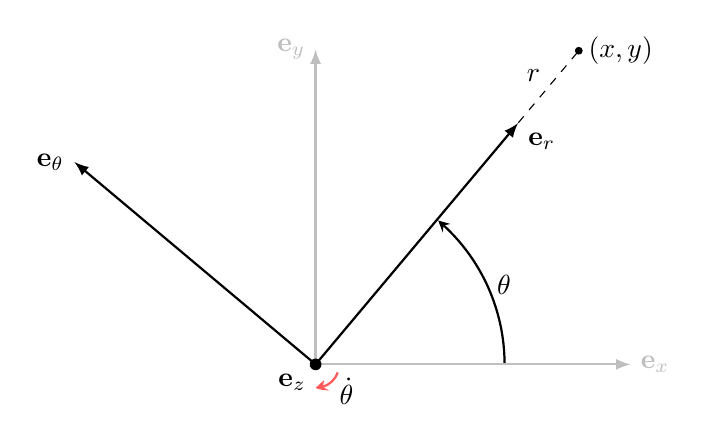
\begin{tikzpicture}[scale=4]
% Draw the polar axes
\pgfmathsetmacro{\radius}{1.3}
\pgfmathsetmacro{\th}{50}
\begin{scope}[rotate=\th]
% Draw the object at (x,y)
\node at (\radius,0) [circle,fill,inner sep=1pt]{};
\node at (\radius, 0)[right]{$(x,y)$};
\draw[thin, dashed] (0,0) -- (\radius,0) node[pos=0.92, left, xshift=-1mm]{$r$};
\draw[->, >=latex, thick] (0,0) -- (1,0) node[anchor=north west]{$\mathbf{e}_r$};
\draw[->, >=latex, thick] (0,0) -- (0,1) node[left]{$\mathbf{e}_\theta$};
\end{scope}

% Draw the angle theta
\pgfmathsetmacro{\rArc}{0.6}
\draw[thick, -{stealth[black]}, black, shorten >=0.5pt] (\rArc,0) arc (0:\th:\rArc) node[pos=0.5, right, black]{$\theta$};
%\draw[thick, path fading=south, shorten >=2pt] (\rArc,0) arc (0:\th:\rArc);

% Draw the normal (x, y) axes
\draw[->, >=latex, thick, black!25] (0,0) -- (1,0) node[right]{$\mathbf{e}_x$};
\draw[->, >=latex, thick, black!25] (0,0) -- (0,1) node[left]{$\mathbf{e}_y$};
\node at (0,0) [circle,fill,inner sep=1.5pt]{};
\node at (0,0) [anchor=north east]{$\mathbf{e}_z$};

% Draw angular velocity
\pgfmathsetmacro{\OmegaArc}{0.075}
\pgfmathsetmacro{\OmegaStartAng}{-20}
\pgfmathsetmacro{\OmegaTotalAng}{-70}
\pgfmathsetmacro{\OmegaAng}{\OmegaStartAng+\OmegaTotalAng}
\draw[thick, -{stealth[bend, red!65]}, red!65] ({\OmegaArc*cos(\OmegaStartAng)},{\OmegaArc*sin(\OmegaStartAng)}) arc (\OmegaStartAng:\OmegaAng:\OmegaArc) node[black, pos=0.8, right, xshift=1mm, yshift=-0.5mm]{$\dot{\theta}$};
\end{tikzpicture}


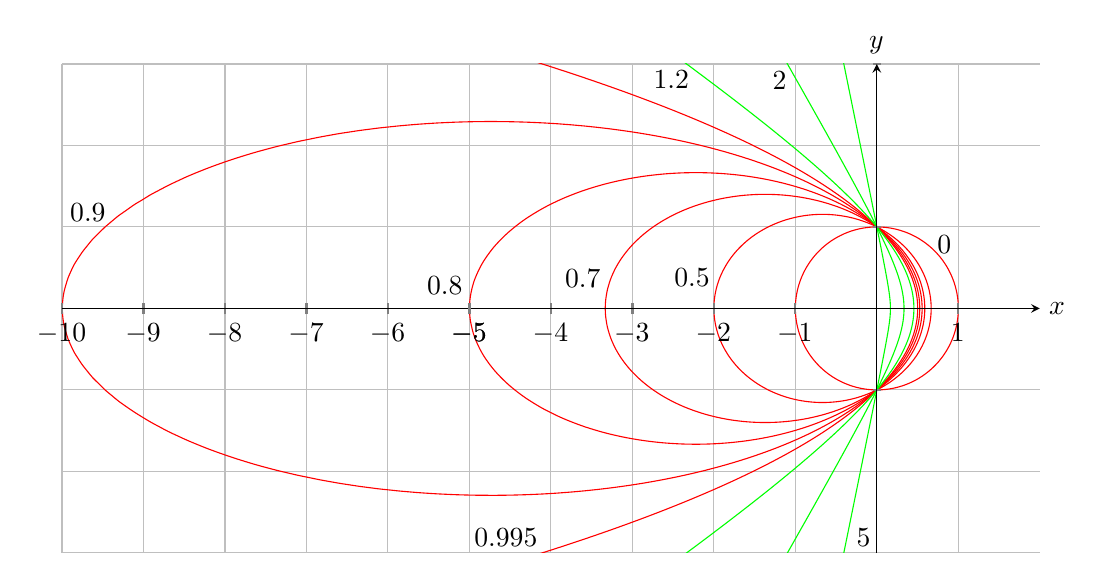
\begin{tikzpicture}
\begin{axis}[width=14cm,
			axis lines=middle,
            axis equal image,
            grid=major,
            xmin=-10, xmax=2,
            ymin=-3, ymax=3,
            xlabel=$x$, xlabel style={right},
            ylabel=$y$, ylabel style={above},
            tick style={thick},
            ticklabel style={font=\normalsize},
            xtick={1,0,...,-20}, extra x ticks={-5}, extra x tick style={grid=none},
            ytick={-5,-4,...,5}, minor ytick={-1,1,...,4},extra y ticks={-2}, extra y tick style={grid=none},
            %xmajorticks=false,
            ymajorticks=false,
            %legend entries={0.5x},
            %        legend style={
            %    at={(0.8,0.937)},
            %    anchor=north,
            %    legend columns=1},
            %    legend cell align={left}
            axis line on top,
        ]
\addplot[data cs=polar,red,domain=0:360,samples=360,smooth] (x, {1/(1 + 0.000*cos(x)))}) node[pos=0.142, right, rotate=0, black]{$0$};
\addplot[data cs=polar,red,domain=0:360,samples=500,smooth] (x, {1/(1 + 0.500*cos(x)))}) node[pos=0.45, left, rotate=0, black]{$0.5$};
\addplot[data cs=polar,red,domain=0:360,samples=500,smooth] (x, {1/(1 + 0.700*cos(x)))}) node[pos=0.465, left, rotate=0, black]{$0.7$};
\addplot[data cs=polar,red,domain=0:360,samples=500,smooth] (x, {1/(1 + 0.8*cos(x)))}) node[pos=0.48, left, rotate=0, black]{$0.8$};
\addplot[data cs=polar,red,domain=0:360,samples=750,smooth] (x, {1/(1 + 0.9*cos(x)))}) node[pos=0.441, left, rotate=0, black, xshift=-1mm]{$0.9$};
\addplot[data cs=polar,red,domain=0:360,samples=360,smooth] (x, {1/(1 + 0.995*cos(x)))}) node[pos=0.9853, above, rotate=0, black, xshift=-3mm]{$0.995$};



\addplot[data cs=polar,green,domain={-acos(-1/1.2)*0.999}:{acos(-1/1.2)*0.999},samples=360,smooth] (x, {1/(1 + 1.2*cos(x)))})  node[pos=0.5000, left, rotate=0, black, xshift=-1mm]{$1.2$};
\addplot[data cs=polar,green,domain={-acos(-1/2)*0.999}:{acos(-1/2)*0.999},samples=360,smooth] (x, {1/(1 + 2*cos(x)))})  node[pos=0.5098, left, rotate=0, black]{$2$};
\addplot[data cs=polar,green,domain={-acos(-1/5)*0.999}:{acos(-1/5)*0.999},samples=360,smooth] (x, {1/(1 + 5*cos(x)))})  node[pos=0.4875, right, rotate=0, black, yshift=-0.25mm]{$5$};
        
%\legend{$f(x)=\sqrt{x} \; {,} \; x \geq 0$ , $g(x)=0.5x$}
\end{axis}
\end{tikzpicture}


\end{document}

% GRAVEYARD
%\newpage
%% kepler_solution
%  \begin{tikzpicture}[scale=4]
%    \coordinate (O) at (0,0);
%    \draw[thick] (-0.1,0) -- (O);
%    \draw[thick] (0,-0.1) -- (O);
%    \draw[->, >=latex, thick] (O) -- (1,0) node[right]{$x$};
%    \draw[->, >=latex, thick] (O) -- (0,1) node[left]{$y$};
%    
%    % Define coordinates of the two bodies
%    \pgfmathsetmacro{\px}{0.85};
%    \pgfmathsetmacro{\py}{0.25};
%    \pgfmathsetmacro{\dx}{0.4};
%    \pgfmathsetmacro{\dy}{0.85};
%    \coordinate (M1) at (\px,\py);
%    \coordinate (M2) at (\dx,\dy);
%    
%    % Draw the bodies
%    \fill[fill=blue!50!black!50] (M1) circle (1pt);
%    \fill[fill=red!50!black!50] (M2) circle (1pt);
%    
%    % Draw the positions of each body relative to the origin
%    \draw[->,>=stealth] (O) -- (M1) node[pos=0.6, below, yshift=0mm]{$\mathbf{r}_1$};
%    \draw[->,>=stealth] (O) -- (M2) node[pos=0.6, left, yshift=-1mm]{$\mathbf{r}_2$};
%    
%    % Draw the vector from body 1 to body 2
%    \draw[->,>=stealth] (M1) -- (M2) node[pos=0.55, right]{$\mathbf{r}$};
%    
%    % Provide the masses
%    \node at (M1) [right, xshift=1mm]{$m_1$};
%    \node at (M2) [left, xshift=-1mm]{$m_2$};
%  \end{tikzpicture}




%\newpage
%% Kepler cylindrical coordinates
%\tdplotsetmaincoords{70}{110}
%  \begin{tikzpicture}[scale=4, tdplot_main_coords]
%	\coordinate (O) at (0,0,0);
%  	\pgfmathsetmacro{\x}{1.5}
%  	\pgfmathsetmacro{\y}{1}
%
%%	% Draw grid to show plane
%%	\begin{scope}[canvas is xy plane at z=0]
%%		\draw[step=0.25,black!20,thin,xshift=0.5cm,yshift=0.5cm] (-1.5*\x,-\y) grid (\x,\y);
%%	\end{scope}    	
%  	
%    \draw[->, >=latex, thick] (O) -- (\x,0,0) node[anchor=north east, yshift=1mm]{$\hat{\mathbf{e}}_x$};
%    \draw[->, >=latex, thick] (O) -- (0,\y,0) node[right]{$\hat{\mathbf{e}}_y$};
%    \draw[->, >=latex, thick] (O) -- (0,0,0.75) node[left]{$\hat{\mathbf{e}}_z$};
%    
%    % Draw polar basis
%    \pgfmathsetmacro{\t}{55}
%    \pgfmathsetmacro{\cost}{cos(\t)}
%    \pgfmathsetmacro{\sint}{sin(\t)}
%    
%    \draw[->, >=latex, thick] (O) -- (\x*\cost,\y*\sint,0) node[anchor=north east, yshift=1mm]{$\hat{\mathbf{e}}_r$};
%    \draw[->, >=latex, thick] (O) -- (-\x*\sint,\y*\cost,0) node[right]{$\hat{\mathbf{e}}_\theta$};
%    
%    \tdplotdefinepoints(0,0,0)(0.5,0,0)(\x*\cost,\y*\sint,0)
%	\tdplotdrawpolytopearc[->, >=stealth]{0.5}{anchor=north,xshift=-0mm, yshift=-0.5mm}{$\theta$}
%  \end{tikzpicture}





%\newpage
%\begin{tikzpicture}[scale=4]
%	\draw[->, >=latex, thick] (0,0) -- (1,0) node[right]{$\hat{\mathbf{e}}_x$};
%	\draw[->, >=latex, thick] (0,0) -- (0,1) node[left]{$\hat{\mathbf{e}}_y$};
%	
%	% Draw polar basis
%    \pgfmathsetmacro{\t}{55}
%    \pgfmathsetmacro{\cost}{cos(\t)}
%    \pgfmathsetmacro{\sint}{sin(\t)}
%    
%    \draw[->, >=latex, thick] (0,0) -- (\cost,\sint) node[anchor=south west, yshift=0mm]{$\hat{\mathbf{e}}_r$};
%    \draw[->, >=latex, thick] (0,0) -- (-\sint,\cost) node[left]{$\hat{\mathbf{e}}_\theta$};
%\end{tikzpicture}









%\newpage
%% Kepler coordinate rotation
%\tdplotsetmaincoords{70}{110}
%  \begin{tikzpicture}[scale=4, tdplot_main_coords]
%  	\coordinate (O) at (0,0,0);
%    \draw[thick] (-1.5,0,0) -- (O);
%    \draw[thick] (0,-1,0) -- (O);
%    \draw[thick] (0,0,-0.75) -- (O);
%    \draw[->, >=latex, thick] (O) -- (1.5,0,0) node[anchor=north east, yshift=1mm]{$X$};
%    \draw[->, >=latex, thick] (O) -- (0,1,0) node[right]{$Y$};
%    \draw[->, >=latex, thick] (O) -- (0,0,0.75) node[left]{$Z$};
%    
%    	\tdplotsetrotatedcoords{60}{-20}{-90}
%    \begin{scope}[tdplot_rotated_coords]
%%    		\draw[thick, black!50] (-1.5,0,0) -- (O);
%%	    \draw[thick, black!50] (0,-1,0) -- (O);
%%	    \draw[thick, black!50] (0,0,-0.75) -- (O);
%    		\draw[->, >=latex, thick, black!50] (O) -- (1,0,0) node[anchor=north east, yshift=1mm]{$x$};
%    		\draw[->, >=latex, thick, black!50] (O) -- (0,1,0) node[right]{$y$};
%	    \draw[->, >=latex, thick, black!50] (O) -- (0,0,1) node[left]{$z$};
%    \end{scope}
%  \end{tikzpicture}